\documentclass[conference]{IEEEtran}
\IEEEoverridecommandlockouts
% The preceding line is only needed to identify funding in the first footnote. If that is unneeded, please comment it out.
%Template version as of 6/27/2024

\usepackage{cite}
\usepackage{amsmath,amssymb,amsfonts}
%\usepackage{algcompatible}
\usepackage{algorithm}
\usepackage{algorithmic}
\usepackage{listings}
\usepackage{comment}
%\usepackage{algpseudocode}
\usepackage{hyperref}
\usepackage{graphicx}
\usepackage{textcomp}
\usepackage{float}
\usepackage{xcolor}
\usepackage{booktabs}
\usepackage{lscape}
\graphicspath{{./images/}}
\def\BibTeX{{\rm B\kern-.05em{\sc i\kern-.025em b}\kern-.08em
    T\kern-.1667em\lower.7ex\hbox{E}\kern-.125emX}}
\begin{document}

\definecolor{codegreen}{rgb}{0,0.6,0}
\definecolor{codegray}{rgb}{0.5,0.5,0.5}
\definecolor{codered}{rgb}{1,0,0}
\definecolor{backcolour}{rgb}{1,1,1}

\lstdefinestyle{style}{
    backgroundcolor=\color{backcolour},   
    commentstyle=\color{codered},
    keywordstyle=\color{orange},
    numberstyle=\tiny\color{codegray},
    stringstyle=\color{codegreen},
    basicstyle=\ttfamily\footnotesize,
    breakatwhitespace=false,         
    breaklines=true,                 
    captionpos=b,                    
    keepspaces=true,                 
    %numbers=left,                    
    numbersep=5pt,                  
    showspaces=false,                
    showstringspaces=false,
    showtabs=false,                  
    tabsize=2
}

\lstset{style=style}

\title{Game Obsession and Player Engagement focused on mobile gaming environments \\
%{\footnotesize \textsuperscript{*}Note: Sub-titles are not captured for https://ieeexplore.ieee.org  and
%should not be used}
%\thanks{Identify applicable funding agency here. If none, delete this.}
}

\author{\IEEEauthorblockN{1\textsuperscript{st} Marshall Sharp}
\IEEEauthorblockA{\textit{Games Academy} \\
\textit{Falmouth University}\\
Falmouth, United Kindgom \\
MS279226@falmouth.ac.uk}
}

\maketitle



\begin{abstract}
Online gaming disorder, or OGA, has become more prevalent in modern times, especially within the research sector. It is up for debate on how we can properly define OGA, how it impacts societal views and/or personal life and how people can mitigate or reduce the impact of OGA. This observation of game addiction and player engagement is studied and analysed from a sample group of 14 people. Through the correlation of time recorded to average play time along with interviewing the participants to see the general view of OGA, as well as gaming habits. The study will also debate about if it should be called Game Obsession and what makes games engaging media. It is found that ultimately, there is insufficient evidence and/or data to prove the hypotheses in full, with experiments using multiple measurements and differing game genres, art styles and sample sizes to gather a more concise reading. 
\end{abstract}
\begin{IEEEkeywords}
engagement, obsession, mobile games
\end{IEEEkeywords}

\section{Introduction}
The nature of addiction, is a difficult thing to define concisely, as we don't know for certain what classifies as an addiction in an age of technological advancements. It is most prevelent in the games industry, with game addiction being classified as a medical condition \cite{NHSHamp24}. This, however, could be flawed, this paper will take a look at game obsession instead of addiction, and go over game addiciton and player enagement based on game obsession instead of addiction, and challenging the classification of such terms. In this paper, an observation will be made, with the main purpose is to find a further understanding of OGA and to gauge if redefinition is required. The variable that will be used for this study is time, both from actual play time and documented play time. The study will also take a look at public perception and views of OGA, and using the data to help answer research questions present in this paper.

\section{Background}
Gaming addiction can be defined in different ways. One paper \cite{yasir2021} defines gaming addiction with the uses and gratification theory and defines overall addiction with the medical paradigm, which has a larger emphasis on biological and psychological dependencies - has been retrofitted to accompany the advancements of technology and specifically in the mobile games industry. This paper also mentions that another study conducted concluded that it can be defined as the regular action of taking drastic actions in the game, such as buying in-game goods or features in a freemium game environment \cite{XWang2021}.S \\

\cite{Naaj2021} was conducted during the midst of the COVID-19 pandemic in early 2020 at Ajman University, where it was found that a sample size of 317 participants participated in an interview, outlining academic and psychological. They were asked three questions: \\

1) "On average, how many hours do you spend playing video games daily?"\\
This question had 17\%  of the participants who didn't play video games, though out of the participants that have, 49\% play around 2 hours on average, with 6\%  playing 8 hours and 3\% playing for 10 hours. The remaining 25\%  for 5 hours as an average daily. Using this information, it can be assumed that gaming addiction affects 9\% if we're only going off of the hours one plays daily. It can be assumed based on this question alone that what causes game addiction is the amount of time played by the participant.\\

2) "Does gaming overall give you a real fulfilment in life?"\\
51\% of the 317 people interviewed said "yes", 10\% felt indifferent, and the remaining 39\% said "no".  This question contradicts question 1 of this study, as the question this poses reevaluates game addiction not based on time played but on the engagement one feels for the game. The \% of people who play for 2 hours is strikingly close to how many people said "yes" to this question, so this could also be used to assume that it's about how enjoyable and engaging the game is, over how much content and playtime is in the game.\\

3) "If it were needed, could you quit playing video games easily?"\\
58\% of the participating body said "yes", whilst 39\% said "no". This gives credence to the assumptions made using question 2, as over half the participants can safely withdraw from gaming entirely. However, with the number of participants who say they can't, it could also be assumed that it can be considered to be somewhat unreliable, as there's no proper discernable evidence to say definitively from the interview conducted.\\ 
 
4)"Did the average daily time you spend playing video games increase during [the] COVID-19 Pandemic?"\\
almost half of those who participated said "no", at 49\%. This also reinforces the assumptions made by question 2, though the volume in the "yes/no" percentage is similar to question 3. It could also be considered inconclusive.

Overall, the interview of participants states that the Average is between 2 hours and 5 hours, Most people find fulfilment in playing games, and it is just as easy to leave gaming as it is to stay, with there being no impact on people's habits over the COVID-19 Pandemic and subsequent lockdowns.\\

Naaj et al. also did ANOVA and T-tests on their hypotheses. All hypotheses revolving around these tests result in their rejection, both with a power of 0 and the same number of participants, but that is where the similarities end. Both tables in the paper revealed that more men play video games, and it does indeed affect the academic level of the students. Table one has a Lower standard deviation and higher mean for men compared to their female counterparts. This is also a similar case in Table 2 of the paper, with females getting equal mean and deviation. This can be seen as there being little to no effect on women when it comes to gaming.\\

ANOVA tests were used to create graphs, which are Figure 2 and Figure 3 for this paper. Both of these factors depict a negative correlation with CGPA. It can be assumed that students who participated in this study have a higher CGPA and spend less time they spend playing video games \cite{Naaj2021}.\\

In Contrast, Rahman et al. 's \cite{Rahman2021} study focused on player engagement. The participants of this paper spent a period of 1.5 hours, up to 4+ hours on games. The most intriguing part of this paper is that even if a participant plays the bare minimum game time that was recorded in the paper, they can still consider themselves addicted to gaming. This compares to \cite{Naaj2021}, who found that the vast majority spent 2 hours playing, which fulfils \cite{Rahman2021} period. Naaj, however, doesn't register the effects of such times played, which Rahman has reported on sleep deprivation, headaches, eye problems, eating disorders, and unhealthy mood swings. The majority of people (28.7\%) slept for 7 hours a day.\\

The effects described in \cite{Rahman2021} may affect one's health despite having no apparent effect on social health. A separate study \cite{Schlagowski2024} found that social health may not be impacted in an online format, which is in contrast to what \cite{NHSHamp24} states. From a medical standpoint, The NHS in Hampshire defines gaming addiction as a variety of symptoms, with the main symptoms being reclusion from the wider world, poor hygiene or lack of attention to basic needs (i.e washing, nourishment such as food or water, or sleep) and hyper fixation on gaming \cite{NHSHamp24}. \cite{Schlagowski2024} found that, despite lacking participants, a first-person view in a social simulator gets more human behaviour. The definition \cite{NHSHamp24} provides can be seen as disagreeable due to the medical paradigm being more on a biological level rather than technological. In addition, it fails to take into consideration other conditions in terms of symptoms, such as ADHD, Autism, and other neurodivergence, which are defined in the text revision of the 5th edition of the Diagnostic and Statistical Manual of Mental Disorders \cite{Association2022}.\\

The concept of High Vulnerability Game Addicts and Low Vulnerability Game Addicts (HVGA and LVGA, respectively) is explored in \cite{Jing2024}'s work, utilising electroencephalography (EEG). EEG consists of technology which allows a researcher to record brain activity and normally takes the form of a headband. HVGA participants are shown to have more than their LVGA compatriots, which is something that is reflected in the results of \cite{Naaj2021}. \cite{Ruqeyya2022} paper also uses EEG, and has a minimun of 80\%  accuracy in it's results. The paper found that player engagement is vital for a mobile game to be successful, with more engagement meriting more success. This contrasts with \cite{Schlagowski2024}, which had barely any impact on player engagement for some players.

The term "Gaming Obsession" could fit this role better. One paper looks into Game Loyalty and Purchase intention \cite{Ramli2022}, in which it was found that Players who are loyal to the games they play are contradictory to a differing source they cited\cite{Widodo2020}, which has a trait of compulsive buying, which mirrors points made in \cite{yasir2021}.  This study was based on 350 out of 680 people, with the majority of the selected amount (65\%) being men and the remaining 35\% being women. The study found that from both of these groups, 55\% of the total play league for 2 -3 hours every day. The NHS  \cite{NHS2021} defines obsession as an "Unwanted or unpleasant thought, image or urge that repeatedly enters your mind, causing feelings of anxiety, disgust or unease," which is in the context of Compulsive Disorder (OCD), though it can be applied to gaming and other external areas.\\

\section{Methodology}
 The experiment will consist of two parts: An artefact which is similar to Cookie Clicker\footnote{\url{https://store.steampowered.com/app/1454400/Cookie_Clicker/}}, using Unity 2023.2.20  \footnote{\url{https://unity.com/}} and stored in this repository:\\

\url{https://github.falmouth.ac.uk/MS279226/Dissertation-MS279226.git}\\

The second part of the experiment is an interview/survey form using Microsoft Forms. Microsoft Forms follows GDPR practice and, due to this, is a safer form application to use when constructing this survey.

\subsection{Artefact}
The Artefact was created as a 2D project, which has a build uploaded to a phone. The game will have a "main" method of creating a point, which could be activated by tapping a large object on the screen. Gathering enough of these points will allow the participant to spend points on various autonomy methods. There will be 4 methods of production that increase in price and point creation. Participants could also stack points, which adds an additive effect to both the output and the cost required to achieve the next addition to the autonomy method. This figure $_{\ref{figure3}}$ prototypes the inner workings of the Artefact. The use will push a button, causing it to increase an integer on a manager up by one, which then displays it on the top of the screen. This is applicable to all buttons on the left hand side. On the right hand side it works similarly, though increases the buttons "quantity" by one if a "threshold" points value is met, which is then deducted from the players score. When the player has played for the appropriate length of time, a transparent button behind the points value will be clicked by the researcher, which will create a Comma Seperated Value (CSV) file and append data into it, or just append the data if a CSV file is already valid.\\

\begin{figure}[H]
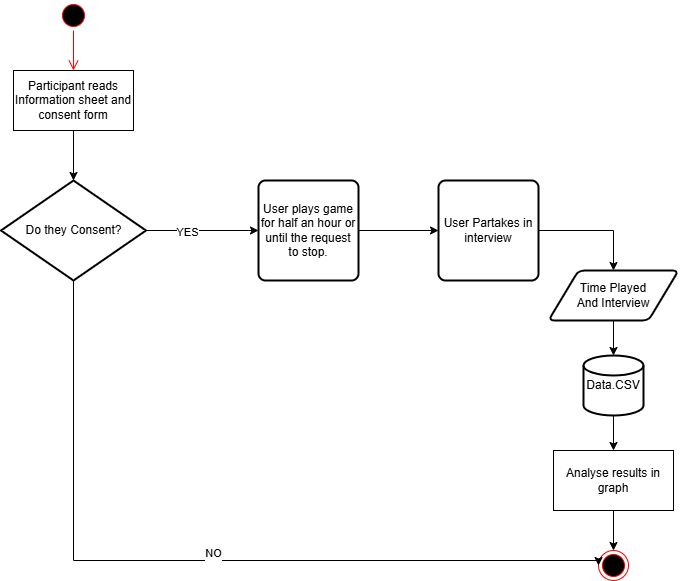
\includegraphics[width = 0.5\textwidth]{UMLProcess}
\caption{A Diagram stating how the experiment will go for a participant}
\label{figure3}
\end{figure}
The UI for such a prototype may look like the following:

\begin{figure}[H]
\begin{center}
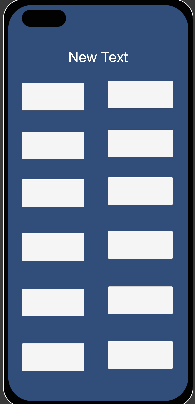
\includegraphics[width = 0.25\textwidth, ]{Sim1}
\caption{A Diagram stating how the experiment may look}
\label{figure1}
\end{center}
\end{figure}


\subsection{Interview/Survey}
The second section of the experiment is an interview/survey that will discuss what the participants liked about the game, what they didn't like, and how they normally go about gaming. This is GDPR compliant. The survey/interview should last around 5 minutes, with a maximum of 20 minutes.

\subsection{Testing}
Unit Testing is conducted throughout the artefact's creation for integers, floats, and bools, among other variables. Unity uses a plug-in that will allow the creation of Unit tests, both in runtime and during editing, with a requirement that there must be an assembly file where the scripts are located, then you can write the tests required. Alongside the Automated Unit tests, there will be a manual walkthrough of the UI and its functionality, both of its requirements and function. The need for stress testing can be done to check for hardware limitations, along with memory leaks, which can go in tandem with the use of the Profiler $_{\ref{Profiler}}$.
\begin{figure}[H]
\begin{center}

\includegraphics[width = 0.5\textwidth, ]{Unittesting}
\caption{Unit testing within the Unity scene}
\label{figure3}
\end{center}
\end{figure}

\begin{figure}[H]
\begin{center}
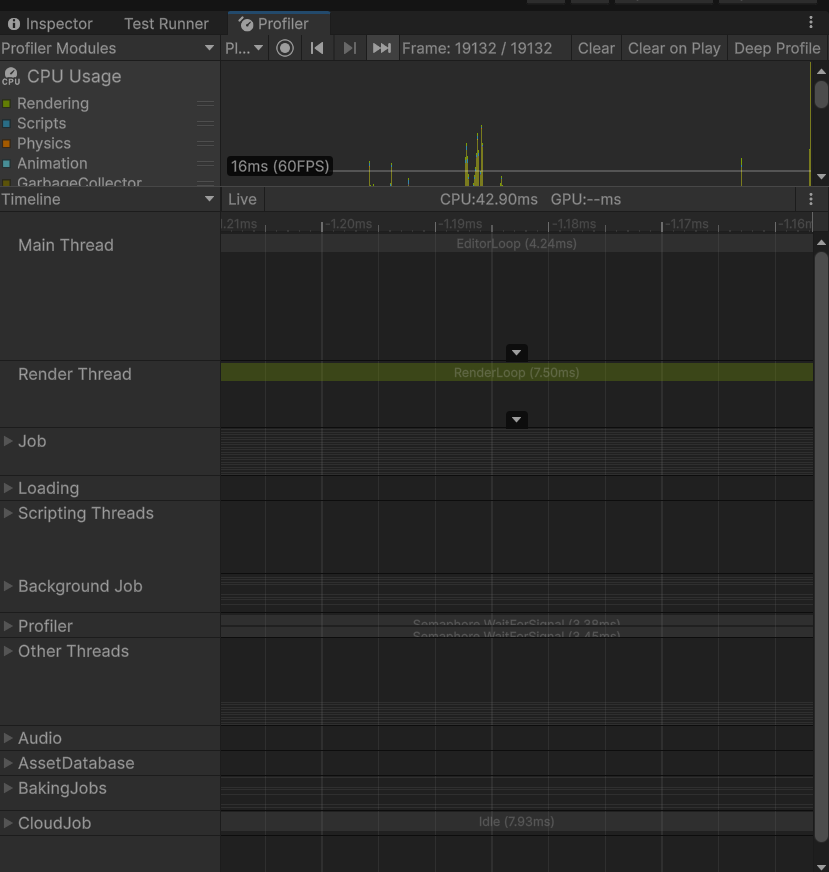
\includegraphics[width = 0.5\textwidth, ]{Profiler}
\caption{Profiler within Unity}
\label{Profiler}
\end{center}
\end{figure}

\subsection{Stats testing}
Utilising G*Power, A T-test using the Point Biseral Model was conducted to determine the sample size for the experiment. Figure 3 shows that the recommended sample size using a large effect size (0.5), a 0.05 error probability and 0.8 Power will result in the sample size being 21.  This is on the smaller end, similar to the paper Ruqeyya wrote \cite{Ruqeyya2022}, which had only 31 participants.  Python will also be used to construct the graphs for time played and compare the time played with the effect of how long, on average, the participant plays games, if any.\\

There is a Null hypothesis in which the player does not focus on the game and sees no reason to continue. This has less than a 5\% chance of occurring. 
\begin{figure}[H]
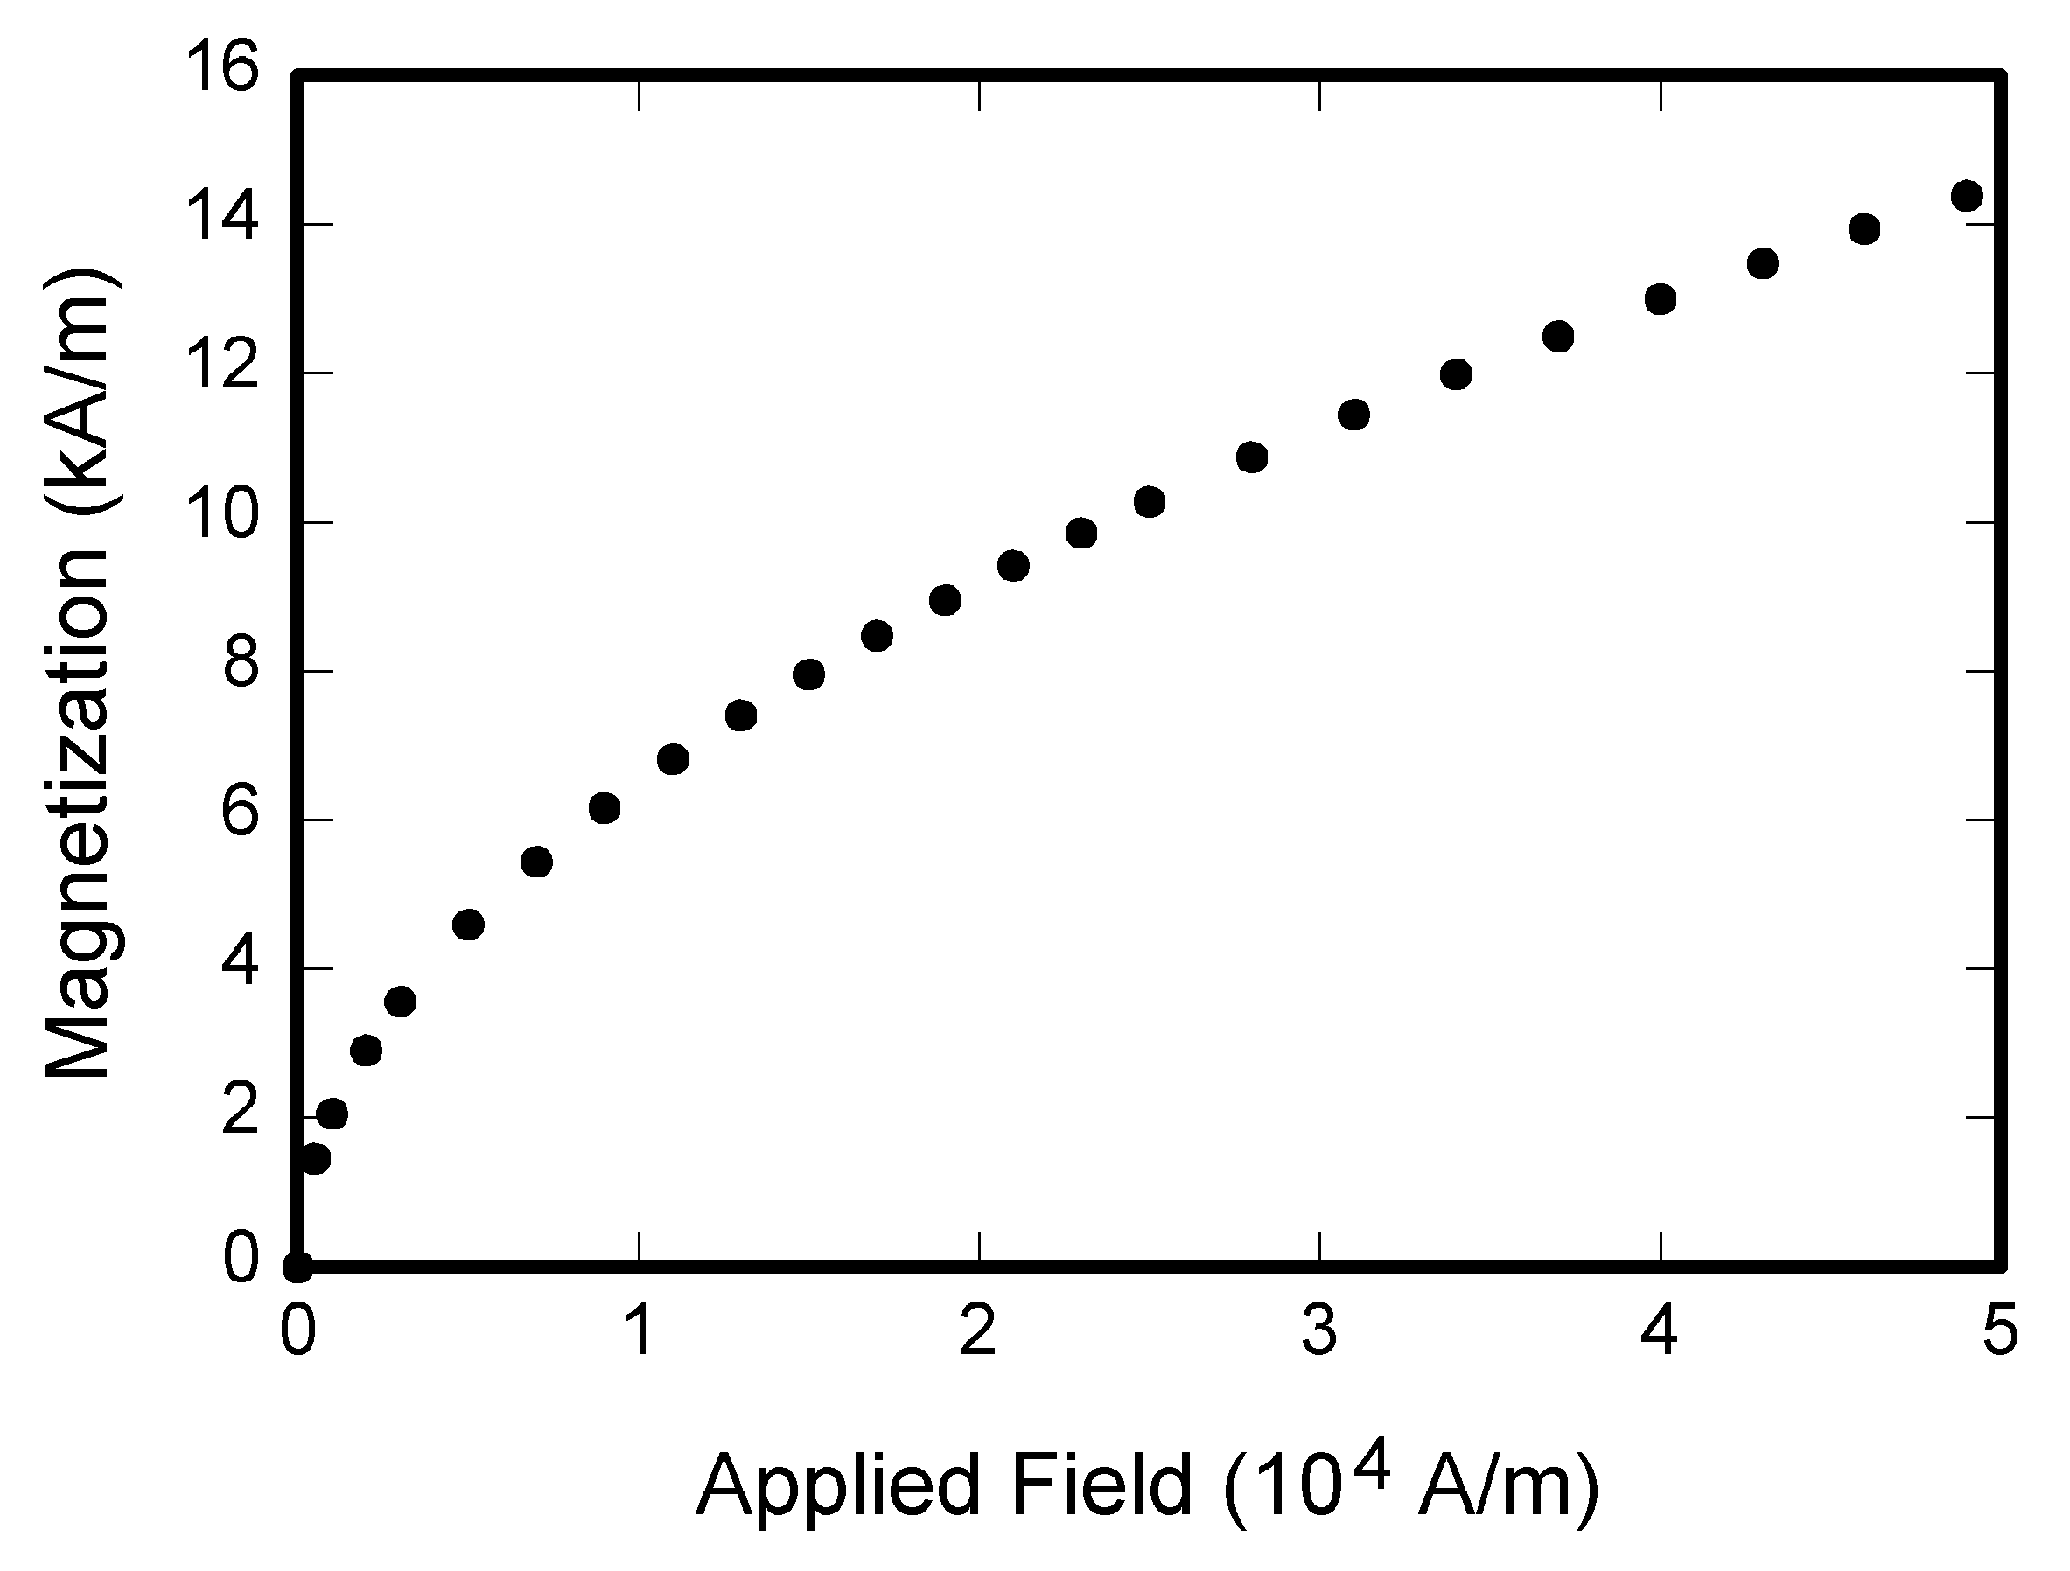
\includegraphics[width =0.5 \textwidth]{fig1}
\caption{The recommended sample size according to the G*Power t-test}
\label{figure4}
\end{figure}

A Graph of the G*Power results was also plotted in the program, which portrays the increase in sample size and its correlation to the Power. This is shown in Figure 4$_{\ref{tab:figure4}}$. In addition, it could be anticipated that the sample size will more accurately be around 20 people due to the restriction of keeping the participants to the university rather than the broader public. 

\begin{figure}[H]
\includegraphics[width = 0.5\textwidth]{fig2}
\caption{The recommended sample size according to the G*Power t-test plotted as a graph, with X as the Power and Y as the sample size}
\label{figure5}
\end{figure}

\subsection{Recording data}
Data will be recorded in a CSV file created by the Application. This file format makes it easier to format into graphs using programming languages such as R and Python. Python, with Pandas, MatPlotlib, Numpy and seaborn would need to be used to create the graphs, as seen in the code below. A method of data collection that could be considered is EEG, which is used in Jing's research \cite{Jing2024} and \cite{Ruqeyya2022}. However, EEG could be seen as invasive, and the institute will not have this equipment. The method chosen will be a more in-person method, manually recording the player's time played through the creation and appendation of the CSV file. If a participant has requested that they no longer want their data used, it will be obfuscated from the analysis and destroyed immediately after. Communication with the participant will be important as well, and contact will be kept once a month if they so request.\\


%\lstinputlisting[language=Python, caption=Python Script for generating Graphs,captionpos=b, firstline=2, lastline=12]{Data_Analysis/Graph.py}

\begin{lstlisting}[language=Python, caption=Python Script for generating Graphs,captionpos=b]
import pandas as pd
import matplotlib.pyplot as plt
import seaborn as sb

csv_data = pd.read_csv("data.csv")

def plotData():
    sb.set_style("darkgrid")
    sb.regplot(x = csv_data["X"],y = csv_data["Y"],data = csv_data,ci=None)
    plt.show()

plotData()
\end{lstlisting}

\subsection{Ethics, RIsk and safety}
There are some things to account for with this research, to do with people and their safety. The experiment is in the hands of the participants, who are required to read an information form and sign a consent form. They could request the experiment to end early if they no longer consent to the experiment.  If they no longer consent, data will not be used for analysis and will be destroyed. Despite there being little physical risk, risk assessments would still need to be carried out, with the removal of items that could be harmful to participants taking part in the research or the addition of items that could mitigate harm/ provide ease of use with the artefact. This paper will adhere to all codes and laws, including the BCS code of conduct\footnote{\url{https://www.bcs.org/media/2211/bcs-code-of-conduct.pdf}} and the Nuremberg code\footnote{\url{https://media.tghn.org/medialibrary/2011/04/BMJ_No_7070_Volume_313_The_Nuremberg_Code.pdf}}. In addition, as an member of the insitute of Falmouth University, I must follow the Research Integrity and Ethics Policy \footnote{\url{https://learningspace.falmouth.ac.uk/pluginfile.php/463699/mod_resource/content/4/Research\%20Integrity\%20and\%20Ethics\%20Policy.pdf}}. 

Enviromentally, Unity utilises C\# as its main programming language, which according to \cite{Jain2020}, A paper comparing multiple languages, namely C++, JAVA, and C\#. The study involves the usage of multiple algorithms and measuring the Wattage used. In this paper, it is found that C\# consumed the least amount of power during runtime, whereas C++ used the most. The scripts made for the artefact will be on the lower end of the power usage. Unity uses a mixture of C++ and C\#, allowing for a more enviromentally friendly engine, with partial access to the source code on github \footnote{\url{https://github.com/Unity-Technologies/UnityCsReference}}.\\

The risks of this experiment are centred around the technology used for the experiment. As it is using a mobile device, caution must be taken if the phone is discovered to be faulty, as such faults could cause the triggering of epilepsy, burns due to the battery, and other injuries caused by the materials of the phone breaking. For this reason, the phone's hardware will be thoroughly inspected and software tested beforehand, with all faulty assets being replaced with a more stable phone. Severe software risks involve the aforementioned triggering of epilepsy, with more common risks including headaches, straining on the eyes and neck, and anxiety. For this reason, usage of software will be limited to half an hour and heavily tested. Whilst some of these scenarios are slim and may not even happen, it is better to be prepared and take measures for these edge cases.\\

Due to the paper's experiment being social and simulating obsession, it is paramount that the half an hour is upheld and is not extended, especially if the participant has any neurodivergence or is considered vulnerable. This will be mentioned as a disclaimer in the information sheet, along with a warning of epilepsy, in case any hardware/software is faulty. This time limit will also reduce the effects of screen use when interacting with the software (headaches, eye strain, etc.). Any failure to adhere is an ethical issue, because of it's nature. \\

\subsection{Questions}
There are two main questions in this research:

 \textbf{Q1: What is the perception of OGA and the related subject?}

 \textbf{Q2: Is there a correlation between perceived time playing a game and Actual time? Is it a sutible measurement for OGA?}\\

\subsection{Hypothesis}
There are two main hypotheses with this experiment, along with a null hypothesis:

H0: The Player will not fulfil any criteria, so there is no change plausible.\\

H0 is in line with Nursafika's paper \cite{Nursafika2024}, which is a study using stumble guys, a competitive party game where you compete in various minigames while being subjected to silly in-game physics. With the use of the Game Experience Questionnaire (GEQ) method, they found that 61.46\% of participants could return to reality after playing the game, 58.30\% felt immersed in the game and 57\% felt the game harmed them, which could be seen as a lesser effect when comparing that result to the 77.28\% of participants who felt the game has had a positive effect on them. At least half of all other values were above 60\%,  with the conclusion that stumble guys have little to no negative impact or addictive nature to players of stumble guys.\\

H1: The Player will have hyperfocus on the game and/or fulfil most of the criteria of game addiction mentioned in \cite{NHSHamp24}, though after being told it's over or requesting, they do not see a reason to keep going.\\

H2: The Player will fulfil the criteria of H1, but will continue with the experiment, even after it's over, either through the duration being up or from requesting it to stop. This will fulfil all of the criteria in \cite{NHSHamp24} and be classed as addiction. \\

Because of the nature of H2, it is an ethical risk if the requirements from the prior subsection aren't adhere'd to.

\subsection {Restraints}
One restraint with this research is the sample size. Due to the sample being students within the university. This limits the findings heavily, with there not being enough to get the sample size that will give a more noteworthy effect. In addition, the sample size will be limited even more due to the period for the experiment only being three weeks. This is a similar pitfall to \cite{Naaj2021} and \cite{Ruqeyya2022}.\\

\subsection{Development Cycle}
%TO DO:  talk about Agile and in what order things were done.
Utilising Agile for this study, 

\section{Results And Discussion}
\begin{table}[H]
\centering
\resizebox{0.5\textwidth}{!}{%
\begin{tabular}{@{}llll@{}}
\toprule
Participant Number & Time Played (minutes) & Average Time Played (minutes) & Hours of Sleep \\ \midrule
1  & 5   & 180 & 9   \\
2  & 10  & 240 & 6   \\
3  & 15  & 270 & 7   \\
4  & 10  & 150 & 7   \\
5  & 4.2 & 540 & 7.5 \\
6  & 5.2 & 240 & 2.5 (not applicable to graphs) \\
7  & 5   & 270 & 5.5 \\
8  & 5.4 & 270 & 7   \\
9  & 5.4 & 180 & 4.5 \\
10 & 5   & 180 & 4.5 \\
11 & 8.6 & 240 & 9   \\
12 & 5.8 & 90  & 6   \\
13 & 4.3 & 120 & 4.5 \\
14 & 15  & 180 & 7.5 \\ \bottomrule
\end{tabular}%
}
\caption{Table 1 - The data collected from the experiment over two weeks.}
\label{data-table}
\end{table}

After conducting the study, the results show a negative correlation.$ _{\ref{data-table}}$ shows the results plotted in the graph below $_{\ref{figure6}}$ in conjunction with the table; the highest time recorded is 540 minutes, or 9 hours, with an average of 225
 minutes, or 3.75 hours. The average time for playing through the study came out to 6 minutes. A reason for this is due to the limitations of the study being very time-sensitive, along with the inability to find the number of participants required by my T-test. Participant 5 is a rather anomalous result due to the high amount of hours put into gaming, as mentioned in the dataset from the interview conducted alongside the artefact, whilst having the lowest recorded time within the dataset. One participant only got 2 -3 hours of sleep, due to chronic insomnia, which has been left out of plotting the graphs, due to the condition causing it not being linked strictly to OGA.

\begin{figure}[H]
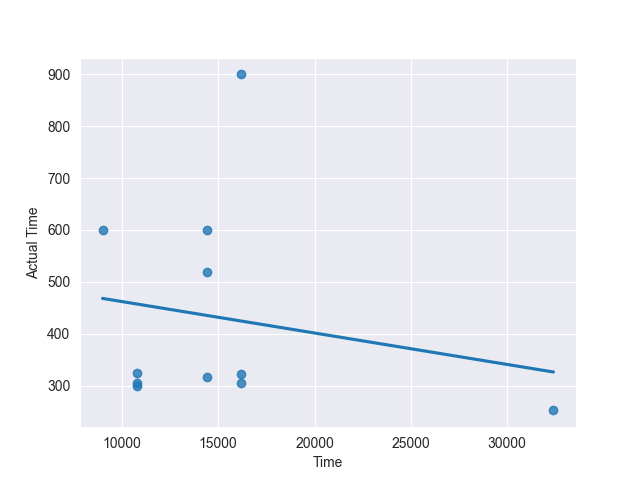
\includegraphics[width = 0.5\textwidth]{Graph1}
\caption{The correlation between perceived time and actual time.}
\label{figure6}
\end{figure}

It is within reason to suspect and accept from the data that H2 is false, whilst there's plausibility that H1 is true. The best solution for clarifying this is to experiment with a larger participant group, along with a longer time frame to conduct the study. H0 could also be plausible, and will be subject to the same solution as H1. Overall, this data is inconclusive, and more work would need to be done regarding this study.

\begin{figure}[H]
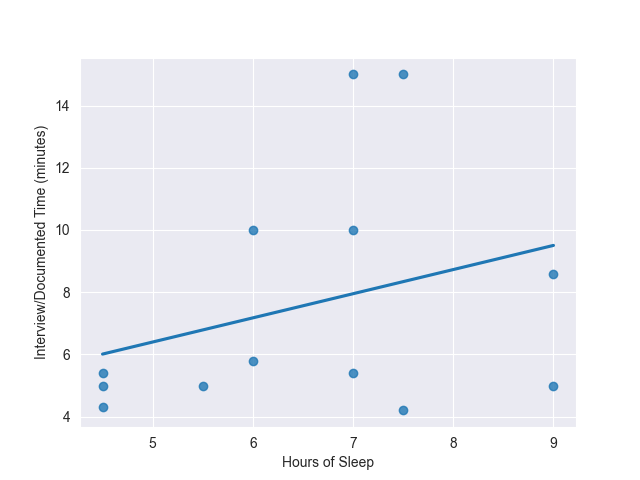
\includegraphics[width = 0.5\textwidth]{Graph2}
\caption{The correlation between perceived time and Sleep.}
\label{figure7}
\end{figure}

There is, however, a correlation between the number of hours a participant sleeps to the amount of time spent playing games. Figure 7$_{\ref{tfigure7}}$ and figure 8$_{\ref{figure8}}$ showcase this change, with the amount of sleep increasing the longer they play games. This is in stark contrast to \cite{Yamazaki2022}, which is a study on general electronics and display screen usage, along with its effect on sleep. The graphs tell the exact opposite of \cite{Yamazaki2022}, and imply that Participants sleep better than if they didn't play/played less.


\begin{figure}[H]
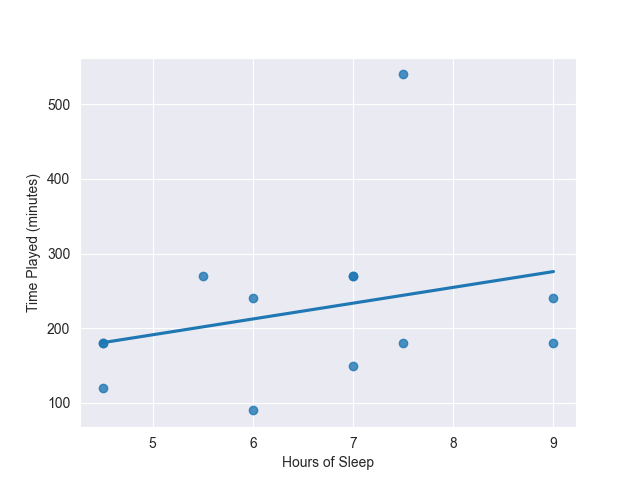
\includegraphics[width = 0.5\textwidth]{Graph3}
\caption{The correlation between Actual time and Sleep}
\label{tab:figure8}
\end{figure}


From the interview, outside of asking about the hours played, some of the questions include:\\

 \textbf{A) When you hear of game addiction, what does your mind immediately think of?}\\

This question spurred many answers about the perception of OGA, with the majority of answers having things in common. The perception of OGA follows Reclusion, prolonged behaviour that is detrimental both to one's health and finances and with that prolonged behaviour, difficulty functioning in society. Other answers exemplify specific game titles, like World of Warcraft, League of Legends, and Final Fantasy 14, which are known to have massive player bases over the years they have been available. Some answers express a generational divide, such as one answer claiming defamatory news articles written by an out-of-touch older generation or grandparents telling them one hour is way too long for a session of video games.\\

One answer out of the Fourteen is an interesting take on the topic: "Just like hobbies, people tend to misinterpret a video game hobby. They claim it's an addiction but it's just a usual thing you love doing." harkens at the fact someone might love what they do with their hobbies to be societally seen as addicted. This answer to this question, whilst opinionated, does show that whilst most people have some form of negative outlook on what OGA is, it could also be argued that, to a lesser extent, is simply the overbearing love for what they enjoy when not dealing with the mundanity of life.\\

 \textbf{B) - The definition of addiction the NHS uses revolves around the use of substances, with its definition being defined as \textit{"not having control over doing, taking or using something to the point where it could be harmful to you"}. Using this definition, does it accurately fit your relation to gaming?}\\

12 ( or 86\%) of the participants answered this question with "no", whilst only 2 (or 14\%) affirmed this definition to their relation with gaming. When asked why, most responses followed a structure of self-control and moderation, though once again highly opinionated. Most answers normally consist of "because I do/have X (where X is a habit used to moderate their time playing video games), I do not believe I suffer from it(OGA).". Interesting answers come from those that affirmed, with "I do stop playing when needed to...When  the game gets good I keep trying to play "one more game"." and "My state with games is using them to keep a healthy state of mind; the issue I have is making sure gaming and gaming-related activities do not become one."\\

The consensus from this question is that you have ways of moderating it, even if creating that moderation seems difficult.\\

 \textbf{C) Do you think "Game Obsession" would be better suited as a name for game addiction? Why?}\\

The Majority of the answers for the question reflect a negatory response, mainly referring to it as a "gateway term" and that addiction is still an ongoing issue. One participant states that it should be treated as an issue separate from OGA, as whilst at the surface level it's the same as any other addiction, it is vastly different to addictions such as substance and gambling.\\

Such questions, along with the data presented, allow the following research questions to be answered:\\

 \textbf{Q1)  What is the perception of OGA and the related subject?}
The perception of OGA and the subject of OGA is seen as an issue that can be regulated with moderation and routine, whilst the common perception of it is normally indicative of poor health and hygiene, the inability to function in a modern society or a popular long-lasting game franchise, series or title. The most conclusive answer to this research question is that the societal view of OGA is seen negatively, either due to generational differences or a common stigma and personification.\\

 \textbf{Q2) Is there a correlation between perceived time playing a game and Actual time? Is it a suitable measurement for OGA?}
There is a correlation between game time and actual time. The speculated result would've been positive, with the higher times mentioned in the interview being seen as higher times played for the game, though the opposite was true, with only a few participants reaching 10+ minutes of playtime and the average being around six minutes. A variety of reasons could exist for this and weren't accounted for, such as the genre of the game or art style, for example. Because of this, there is a weak and negative correlation with this measurement.

\section{Conclusion}
%TO DO:  Link back to research, add meaning and defend findings.
Overall in this paper, a study was conducted about OGA and Player engagement, utilising an Idle simulation game and interview. From a participation group of 14 people over 48 hours, there was a weak and negative correlation between the player's sense of time and the player's mentioned time. There is, however, a correlation between Time spent playing games and the number of hours of sleep a participant has, showing a positive correlation between the time played and the sleep each participant gets. This paper discussed and researched Game addiction and what defines Game Addiction, both using the medical paradigm and from the public view. Moving forward, this experiment could be attempted again, with differing game genres, art styles, study periods and sample sizes.

\bibliographystyle{IEEEtran}
\bibliography{Dissertationbib.bib} 
\section {Addendum - Reflection}
Throughout this study, I have had, in hindsight, multiple issues within it, mainly regarding the six subsections listed below. Looking back and my willingness to go into the games industry, this study has taught me a lot about not only development cycles but the documentation of said development cycles, along with teaching me new skills, such as unit testing, file creation and the academic process.
\subsection{Cognitive}
Throughout this study, one issue I had was gathering and recalling the data for the background, either due to not knowing where to look, forgetting where to look or how to properly comprehending some of the topics and methods within the papers found. To this end, it made producing the background difficult and tedious. Starting from April 11th until 23rd December 2025, I will look into the concepts presented not only in the papers found for this paper but other papers as well in regard to methodologies. 

%S - Specific:
%M - Measureable:
%A- Achievable: 
%R - Relevance:
%T - Time:

\subsection{Methodological}
Methodologically, the most difficult thing for me to do in this study was stats testing and using G*power. Figuring out what test to use and the various parameters that can be applicable was the hardest thing for me to understand. Going forward and in any future studies, I will do extensive research on what each of the statistical analysis tests do, what they are commonly used for and what variables I am looking for when determining sample size or null hypothesis

%S - Specific
%M - Measureable:
%A- Achievable: 
%R - Relevance:
%T - Time:
\subsection{Affective}
Looking back on this study, I found myself to be calm over the creation of the artefact. There is not much else to say
%S - Specific
%M - Measureable:
%A- Achievable: 
%R - Relevance:
%T - Time:
\subsection{Dispositional}
%S - Specific
%M - Measureable:
%A- Achievable: 
%R - Relevance:
%T - Time:
\subsection{Interpersonal}
%S - Specific
%M - Measureable:
%A- Achievable: 
%R - Relevance:
%T - Time:
\subsection{Practice}
%S - Specific
%M - Measureable:
%A- Achievable: 
%R - Relevance:
%T - Time:
\begin{comment}
\section{Addendum - Figures, Graphs and tables}

\begin{figure}[H]
\begin{center}
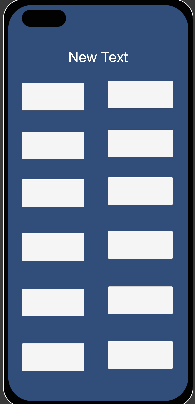
\includegraphics[width = 0.25\textwidth, ]{Sim1}
\caption{A Diagram stating how the experiment may look}
\label{tab:figure1}
\end{center}
\end{figure}

\begin{figure}[H]
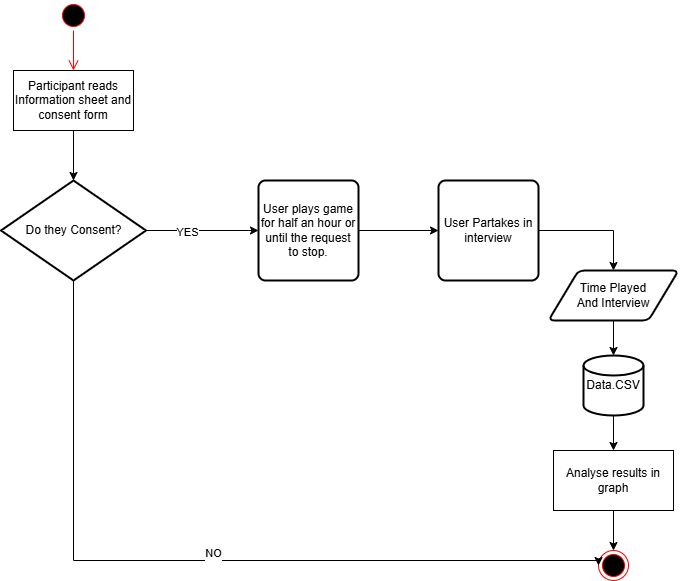
\includegraphics[width = 0.5\textwidth]{UMLProcess}
\caption{A Diagram stating how the experiment will go for a participant}
\label{tab:figure2}
\end{figure}

\begin{figure}[H]
\begin{center}

\includegraphics[width = 0.5\textwidth, ]{Unittesting}
\caption{Unit testing within the Unity scene}
\label{tab:figure3}
\end{center}
\end{figure}

\begin{figure}[H]
\begin{center}
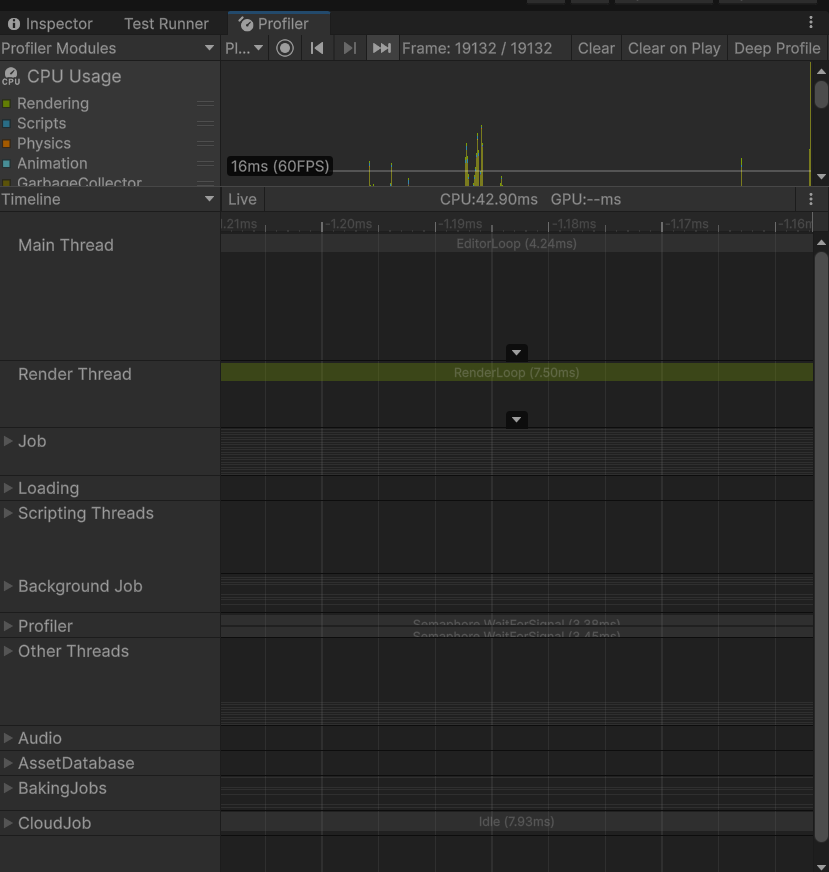
\includegraphics[width = 0.5\textwidth, ]{Profiler}
\caption{Profiler within}
\label{tab:Profiler}
\end{center}
\end{figure}

\begin{figure}[H]
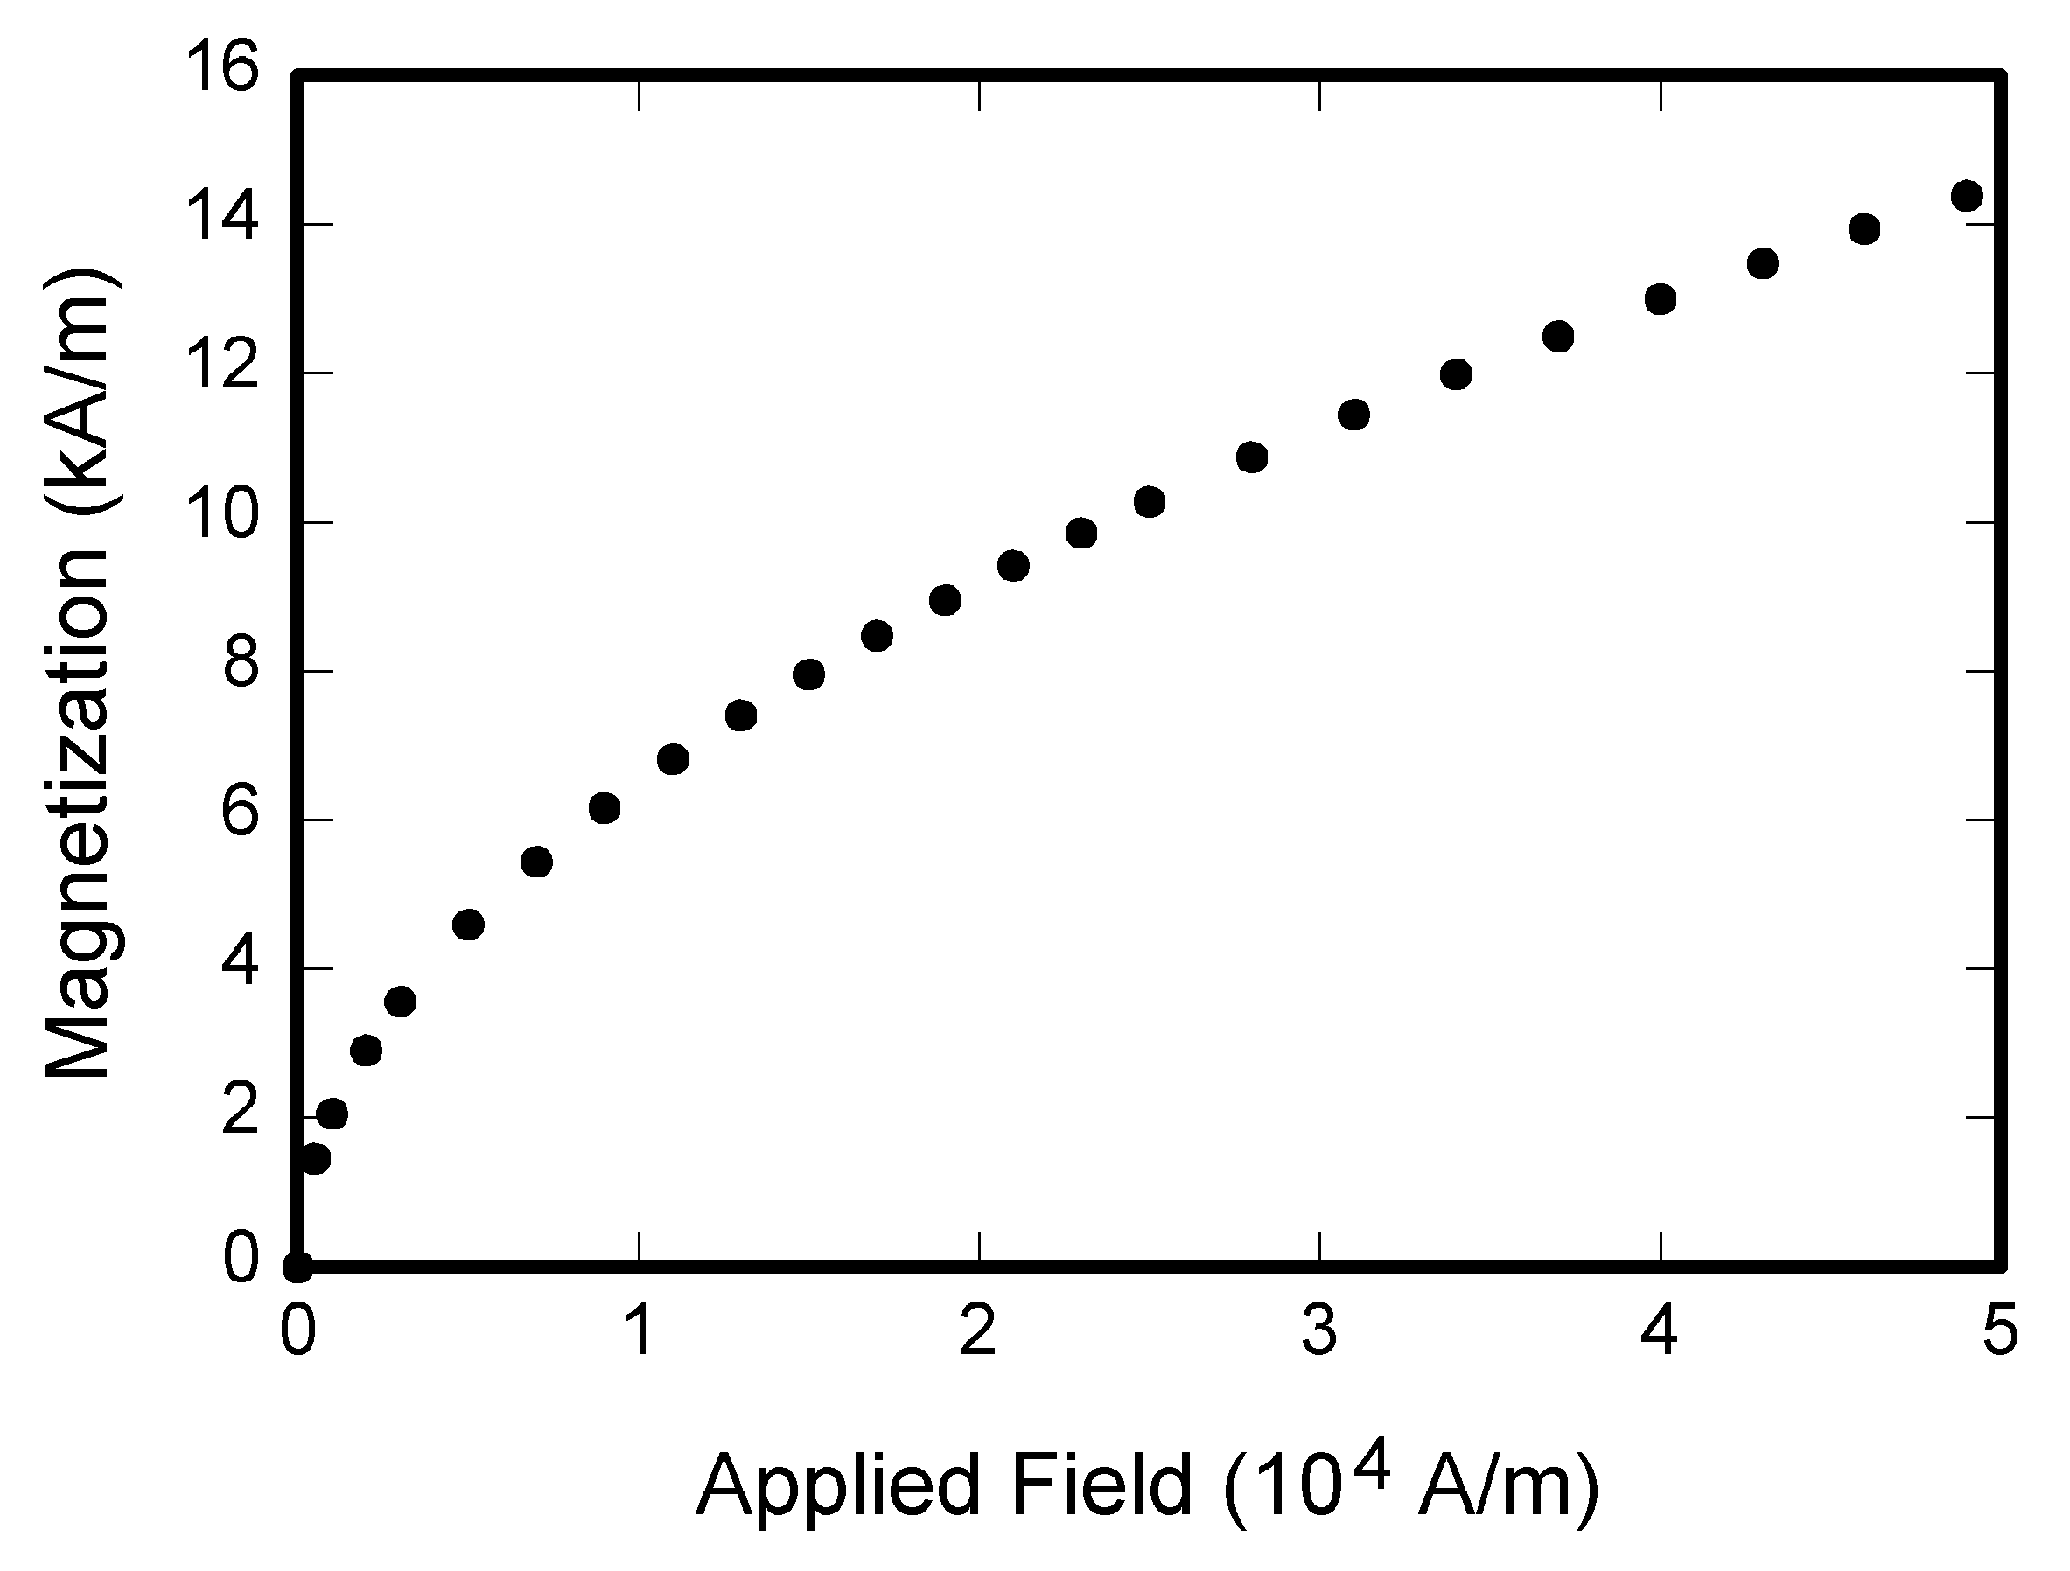
\includegraphics[width =0.5 \textwidth]{fig1}
\caption{The recommended sample size according to the G*Power t-test}
\label{tab:figure4}
\end{figure}

\begin{lstlisting}[language=Python, caption=Python Script for generating Graphs,captionpos=b]
import pandas as pd
import matplotlib.pyplot as plt
import seaborn as sb

csv_data = pd.read_csv("data.csv")

def plotData():
    sb.set_style("darkgrid")
    sb.regplot(x = csv_data["X"],y = csv_data["Y"],data = csv_data,ci=None)
    plt.show()

plotData()
\end{lstlisting}

\begin{figure}[H]
\includegraphics[width = 0.5\textwidth]{fig2}
\caption{The recommended sample size according to the G*Power t-test plotted as a graph, with X as the Power and Y as the sample size}
\label{tab:figure5}
\end{figure}

\begin{table}[H]
\centering
\resizebox{0.5\textwidth}{!}{%
\begin{tabular}{@{}llll@{}}
\toprule
Participant Number & Time Played (minutes) & Average Time Played (minutes) & Hours of Sleep \\ \midrule
1  & 5   & 180 & 9   \\
2  & 10  & 240 & 6   \\
3  & 15  & 270 & 7   \\
4  & 10  & 150 & 7   \\
5  & 4.2 & 540 & 7.5 \\
6  & 5.2 & 240 &  N/A  \\
7  & 5   & 270 & 5.5 \\
8  & 5.4 & 270 & 7   \\
9  & 5.4 & 180 & 4.5 \\
10 & 5   & 180 & 4.5 \\
11 & 8.6 & 240 & 9   \\
12 & 5.8 & 90  & 6   \\
13 & 4.3 & 120 & 4.5 \\
14 & 15  & 180 & 7.5 \\ \bottomrule
\end{tabular}%
}
\caption{Table 1 - The data collected from the experiment over two weeks.}
\label{tab:data-table}
\end{table}

\begin{figure}[H]
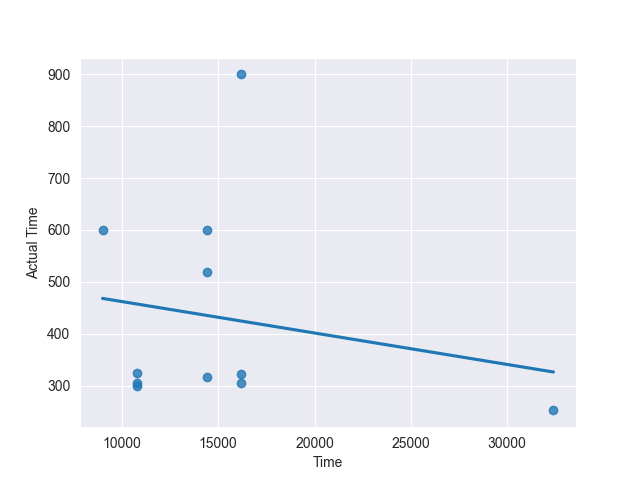
\includegraphics[width = 0.5\textwidth]{Graph1}
\caption{The correlation between perceived time and actual time.}
\label{tab:figure6}
\end{figure}

\begin{figure}[H]
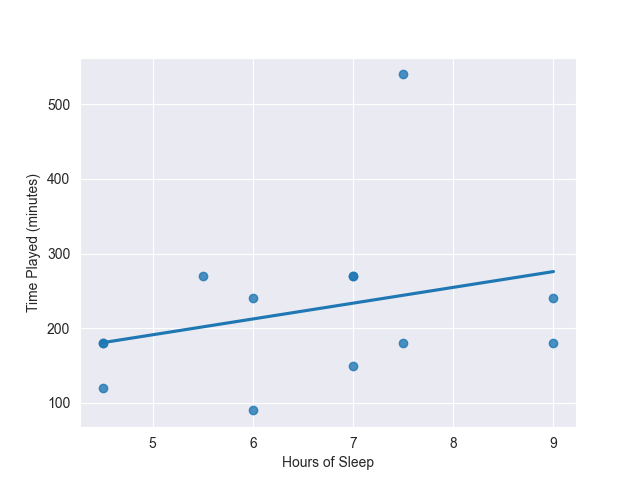
\includegraphics[width = 0.5\textwidth]{Graph3}
\caption{The correlation between Actual time and Sleep}
\label{tab:figure8}
\end{figure}
\end{comment}
\end{document}
